\chapter{Strings and Csets}

\textsc{Perspective}: Several aspects of strings as a language feature
in Icon have a strong influence on how they are handled by the
implementation. First of all, strings are the most frequently used
type of data in the majority of Icon programs. The number of different
strings and the total amount of string data often are
large. Therefore, it is important to be able to store and access
strings efficiently.

Icon has many operations on strings---nearly fifty of them. Some
operations, such as determining the size of a string, are performed
frequently. The efficiency of these operations is an important issue
and influences, to a considerable extent, how strings are represented.

Icon strings may be very long. Although some limitation on the maximum
length of a string may be acceptable as a compromise with the
architecture of the computer on which Icon is implemented (and hence
considerations of efficiency), this maximum must be so large as to be
irrelevant for most Icon programs.

String lengths are determined dynamically during program execution,
instead of being specified statically in declarations. Much of the
advantage of string processing in Icon over other programming
languages comes from the automatic management of storage for strings.

Any of the 256 8-bit ASCII characters can appear in an Icon
string. Even the {\textquotedbl}null{\textquotedbl} character is
allowed.

Several operations in Icon return substrings of other
strings. Substrings tend to occur frequently, especially in programs
that analyze (as opposed to synthesize) strings.


Strings in Icon are atomic---there are no operations in Icon that
change the characters in existing strings. This aspect of Icon is not
obvious; in fact, there are operations that appear to change the
characters in strings. The atomic nature of string operations in Icon
simplifies its implementation considerably. For example, assignment of
a string value to a variable need not (and does not) copy the string.

The order in which characters appear is an essential aspect of
strings. There are many situations in Icon, however, where several
characters have the same status but where their order is
irrelevant. For example, the concepts of vowels and punctuation marks
depend on set membership but not on order. Csets are provided for such
situations. Interestingly, many computations can be performed using
csets that have nothing to do with the characters themselves (Griswold
and Griswold 1983, pp. 181-191).


\section[5.1 Strings]{5.1 Strings}
\subsection[5.1.1 Representation of Strings]{5.1.1 Representation of Strings}

Although it may appear natural for the characters of a string to be
stored in consecutive bytes, this has not always been so. On earlier
computer architectures without byte addressing and character
operations, some string-manipulation languages represented strings by
linked lists of words, each word containing a single character. Such a
representation seems bizarre for modem computer architectures and
obviously consumes a very large amount of memory-an intolerable amount
for a language like Icon.

The C programming language represents strings (really arrays of
characters) by successive bytes in memory, using a zero (null) byte to
indicate the end of a string. Consequently, the end of a string can be
determined from the string itself, without any external
information. On the other hand, determining the length of a string, if
it is not already known, requires indexing through it, incrementing a
counter until a null byte is found. Furthermore, and very important
for a language like Icon, substrings (except terminal ones) cannot
occur within strings, since every C string must end with a null byte.

Since any character can occur in an Icon string, it is not possible to
use C's null-termination approach to mark ends of strings. Therefore,
there is no way to detect the end of a string from the string itself,
and there must be some external way to determine where a string
ends. This consideration provides the motivation for the qualifier
representation described in the last chapter. The qualifier provides
information, external to the string itself, that delimits the string
by the address of its first character and its length. Such a
representation makes the computation of substrings fast and
simple---and, of course, determining the length of a string is
fast and independent of its length.

Note that C-style strings serve perfectly well as Icon-style strings;
the null byte at the end of a C-style string can be ignored by
Icon. This allows strings produced by C functions to be used by
Icon. The converse is not true; in order for an Icon string to be used
by C, a copy must be made with a null byte appended at the end.

Some strings are compiled into the run-time system and others, such as
strings that appear as literals in a program, are contained in icode
files that are loaded into memory when program execution
begins. During program execution, Icon strings may be stored in work
areas (usually referred to as
{\textquotedbl}buffers{\textquotedbl}). Most newly created strings,
however, are allocated in a common string region.

As source-language operations construct new strings, their characters
are appended to the end of those already in the string region. The
amount of space allocated in the string region typically increases
during program execution until the region is full, at which point it
is compacted by garbage collection, squeezing out characters that are
no longer needed. See Chapter 11 for details.

In the previous chapter, the string to which a qualifier points is
depicted by an arrow followed by the string. For example, the string
{\textquotedbl}the{\textquotedbl} is represented by the qualifier

\begin{picture}(300,50)(0,8)
\put(100,10){\dvboxptr{3}{}{50}{"the"}}
\end{picture}

The pointer to {\textquotedbl}the{\textquotedbl} is just a notational
convenience. A more accurate representation is

\begin{picture}(300,80)(0,8)
\put(100,40){\dvbox{3}{}{}}
\put(100,40){\rdptr{72}{18}}
\put(233,20){ ...  t h e  ...}
\end{picture}

The actual value of the v-word might be 0x569a (hexadecimal), where
the character t is at memory location 0x569a, the character h is at
location 0x569b, and the character e is at location 0x569c.

\subsection[5.1.2 Concatenation]{5.1.2 Concatenation}

In an expression such as

\iconline{
\ \ s := "hello"
}

\noindent the string {\textquotedbl}hello{\textquotedbl} is contained
in data provided as part of the icode file, and a qualifier for it is
assigned to s; no string is constructed. Some operations that produce
strings require the allocation of new strings. Concatenation is a
typical example:

\iconline{
\ \ s1 := "ab" || "cdef"
}

\noindent In this expression, the concatenation operation allocates
space for six characters, copies the two strings into this space, and
produces a qualifier for the result:

%% 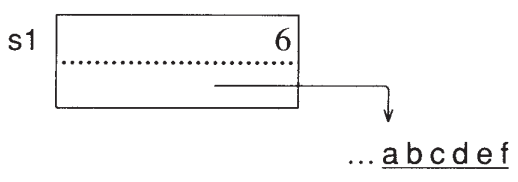
\includegraphics[width=2.6783in,height=0.9366in]{ib-img/ib-img020.png}
\begin{picture}(300,80)(0,8)
\put(100,40){\dvbox{6}{}{}}
\put(100,40){\tlboxlabel{s1}}
\put(100,40){\rdptr{72}{18}}
\put(233,20){ ...  \underline{abcdef}  ...}
\end{picture}

This qualifier then becomes the value of \texttt{s1}.

There are important optimizations in concatenation. If the first
argument in a concatenation is the last string in the string region,
the second argument is simply appended to the end of the string
region. Thus, operations of the form

\iconline{
\ \ s := s || \textit{expr}
}

\noindent perform less allocation than operations of the form

\iconline{
\ \ s := \textit{expr }|| s
}

Similarly, if the strings being concatenated are already adjacent, no
concatenation need be performed. Except for these optimizations, no
string construction operation attempts to use another instance of a
string that may exist somewhere else in the string region. As a
result,

\iconcode{
\> s1 := "ab" || "c"\\
\> s2 := "a" || "bc"
}

\noindent produce two distinct strings:

\begin{picture}(300,120)(0,8)
\put(100,80){\dvbox{3}{}{}}
\put(100,80){\tlboxlabel{s2}}
\put(100,80){\rdptr{92}{58}}
\put(100,40){\dvbox{3}{}{}}
\put(100,40){\tlboxlabel{s1}}
\put(100,40){\rdptr{72}{18}}
\put(233,20){ ...  \underline{abc}\hspace{2pt}\underline{abc}  ...}
\end{picture}

The RTL code for the concatenation operation is

\iconcode{
\>operator\{1\} || cater(x,y)\\
\>if !cnv:string(x) then\\
\>\>runerr(103, x)\\
\>if !cnv:string(y) then\\
\>\>runerr(103, y)\\
\\
\>abstract \{\\
\>\>return string\\
\>\>\}\\
\>body \{\\
\>\>CURTSTATE();\\
\\
\>\>/*\\
\>\>\ * \ Optimization 1: \ The strings to be concatenated are\\
\>\>\ * \ already adjacent in memory; no allocation is required.\\
\>\>\ */\\
\>\>if (StrLoc(x) + StrLen(x) == StrLoc(y)) \{\\
\>\>\>StrLoc(result) = StrLoc(x);\\
\>\>\>StrLen(result) = StrLen(x) + StrLen(y);\\
\>\>\>return result;\\
\>\>\>\}\\
\>\>else if ((StrLoc(x) + StrLen(x) == strfree)\\
\>\>\&\& (DiffPtrs(strend,strfree) > StrLen(y))) \{\\
\>\>\>/*\\
\>\>\>\ * Optimization 2: The end of x is at the end of the string space.\\
\>\>\>\ * \ Hence, x was the last string allocated and need\\
\>\>\>\ * \ not be re-allocated. y is appended to the string\\
\>\>\>\ * \ space and the result is pointed to the start of x.\\
\>\>\>\ */\\
\ \  result = x;\\
\ \  /*\\
\ \  \ * Append y to the end of the string space.\\
\ \  \ */\\
\ \  Protect(alcstr(StrLoc(y),StrLen(y)), runerr(0));\\
\ \  /*\\
\ \  \ * \ Set the length of the result and return.\\
\ \  \ */\\
\ \  StrLen(result) = StrLen(x) + StrLen(y);\\
\ \  return result;\\
\>\>\>\}\\
\\
\>\>/*\\
\>\>\ * Otherwise, allocate space for x and y, and copy them\\
\>\>\ * \ to the end of the string space.\\
\>\>\ */\\
\>\>Protect(StrLoc(result) = alcstr(NULL, StrLen(x) + StrLen(y)), runerr(0));\\
\>\>memcpy(StrLoc(result), StrLoc(x), StrLen(x));\\
\>\>memcpy(StrLoc(result) + StrLen(x), StrLoc(y), StrLen(y));\\
\\
\>\>/*\\
\>\>\ * \ Set the length of the result and return.\\
\>\>\ */\\
\>\>StrLen(result) = StrLen(x) + StrLen(y);\\
\>\>return result;\\
\>\>\}\\
end
}

The function \texttt{strreq(n)} assures that there are at least
\texttt{n} bytes available in the allocated string region. See Chapter
11 for details. The function \texttt{alcstr(s, n)} allocates
\texttt{n} characters and copies \texttt{s} to that space. The global
variable \texttt{strfree} points to the beginning of the free space at
the end of the allocated string region.

\subsection[5.1.3 Substrings]{5.1.3 Substrings}

Many string operations do not require the allocation of a new string
but only produce new qualifiers. For example, if the value of
\texttt{s1} is \texttt{{\textquotedbl}abcdef{\textquotedbl}}, the
substring formed by

\iconline{
\>s2 := s1[3:6]
}

\noindent does not allocate a new string but only produces a qualifier
that points to a substring of \texttt{s1}:



\begin{picture}(300,120)(0,8)
\put(100,80){\dvbox{3}{}{}}
\put(100,80){\tlboxlabel{s2}}
\put(100,80){\rdptr{85}{58}}
\put(100,40){\dvbox{6}{}{}}
\put(100,40){\tlboxlabel{s1}}
\put(100,40){\rdptr{72}{18}}
\put(233,20){ ...  \underline{abcdef}  ...}
\put(265,16){\line(1,0){16}}
\end{picture}

In order for Icon string values to be represented in memory by
substrings, it is essential that there be no Icon operation that
changes the characters inside a string. As mentioned earlier, this is
the case, although it is not obvious from a cursory examination of the
language. C, on the other hand, allows the characters in a string to
be changed. The difference is that C considers a string to be an array
of characters and allows assignment to the elements of the array,
while Icon considers a string to be an indivisible atomic object. It
makes no more sense in Icon to try to change a character in a string
than it does to try to change a digit in an integer. Thus, if

\iconline{
\>i := j
}

and

\iconline{
\>j := j + 1
}

\noindent the value of \texttt{i} does not change as a result of the
subsequent assignment to \texttt{j}. So it is with strings in Icon.

Admittedly, there are operations in Icon that \textit{appear }to
change the characters in a string. For example,

\iconline{
\>s1[3] := "x"
}

\noindent gives the appearance of changing the third character in
\texttt{s1} to \texttt{{\textquotedbl}x{\textquotedbl}}.  However,
this expression is simply shorthand for

\iconline{
\>s1 := s1[1:3] || "x" || s1[4:0]
}

A new string is created by concatenation and a new qualifier for it is
assigned to \texttt{s1}, as shown by

\begin{picture}(300,120)(0,8)
\put(100,80){\dvbox{6}{}{}}
\put(100,80){\tlboxlabel{s1}}
\put(100,80){\rdptr{107}{58}}
\put(100,40){\dvbox{3}{}{}}
\put(100,40){\tlboxlabel{s2}}
\put(100,40){\rdptr{85}{18}}
\put(233,20){ ...  ab\underline{cde}f\hspace{2pt}\underline{abxdef}  ...}
\end{picture}

Of course, the length of the string may be increased or decreased by
assignment to a substring, as in

\iconcode{
\>s1[3] := "xxx"\\
\>s1 [2:5] := ""
}

\subsection[5.1.4 Assignment to Subscripted Strings]{5.1.4 Assignment to Subscripted Strings}

Expressions such as \texttt{x[i]} and \texttt{x[i:j]} represent a
particular challenge in the implementation of Icon. In the first
place, the translator cannot determine the type of x. In the case of
\texttt{x[i]}, there are four basic types that \texttt{x} may
legitimately have: string, list, table, and record. Of course, any
type that can be converted to a string is legitimate
also. Unfortunately, the \textit{nature }of the operation, not just
the details of its implementation, depends on the type. For strings,

\iconline{
\>s1 [3] := s2
}

\noindent replaces the third character of \texttt{s1} by \texttt{s2}
and is equivalent to concatenation, as described previously.  For
lists, tables, and records,

\iconline{
\>x[3] := y
}

\noindent changes the third \textit{element }of \texttt{x} to
\texttt{y}{}--quite a different matter (see Exercise 5.5).

This problem is pervasive in Icon and only needs to be noted in
passing here. The more serious problem is that even if the subscripted
variable is a string, the subscripting expression has different
meanings, depending on the context in which it appears.

If \texttt{s} is a variable, then \texttt{s[i]} and \texttt{s[i:j]}
also are variables. In a dereferencing context, such as

\iconline{
\>write(s[2:5])
}

\noindent the result produced by \texttt{s[2:5]} is simply a substring
of \texttt{s}, and the subscripting expression produces the
appropriate qualifier.

Assignment to a subscripted string, as in

\iconline{
\>s[2:5] := "xxx"
}

\noindent is not at all what it appears to be superficially. Instead,
as already noted, it shorthand for an assignment to \texttt{s}:

\iconline{
\>s := s[1] || "xxx" || s[6:0]
}

If the translator could determine whether a subscripting expression is
used in dereferencing or assignment context, it could produce
different code for the two cases. As mentioned in Sec. 4.3.2, however,
the translator cannot always make this determination. Consequently,
trapped variables are used for subscripted strings much in the way they
were used for keywords in Icon Version 6. For example, if the value of \texttt{s} is
\texttt{{\textquotedbl}abcdef{\textquotedbl}}, the result of
evaluating the subscripting expression \texttt{s[2:5]} is a
\textit{substring trapped variable} that has the form

\begin{picture}(300,170)
\put(140,0){\dvbox{}{npv}{}}
\put(140,0){\tlboxlabel{\texttt{s}}}
\put(140,0){\ruptr{30}{48}}
\put(140,48){\dvboxptr{}{npv}{50}{}}
\put(140,80){\blkbox{3}{2}}
\put(140,80){\rightboxlabels{length}{offset}}
\put(140,112){\wordbox{tvsubs}{}}
\put(10,112){\dvboxptr{tvsubs}{nptv}{50}{}}
\put(10,112){\tlboxlabel{\texttt{s[2:5]}}}
\put(260,32){\dvboxptr{6}{}{50}{"abcdef"}}
\end{picture}

Note that both the variable for \texttt{s} and the variable in the
substring trapped-variable block point to the same value. This makes
it possible for assignment to the substring trapped variable to change
the value of \texttt{s}.

The length and offset of the substring provide the necessary
information either to produce a qualifier for the substring, in case
the subscripting expression is dereferenced, or to construct a new
string in case an assignment is made to the subscripting
expression. For example, after an assignment such as

\iconline{
\>s[2:5] := "x"
}

\noindent the situation is

\begin{picture}(300,170)
\put(140,0){\dvbox{}{npv}{}}
\put(140,0){\tlboxlabel{\texttt{s}}}
\put(140,0){\ruptr{30}{48}}
\put(140,48){\dvboxptr{}{npv}{50}{}}
\put(140,80){\blkbox{1}{2}}
\put(140,80){\rightboxlabels{length}{offset}}
\put(140,112){\wordbox{tvsubs}{}}
\put(10,112){\dvboxptr{tvsubs}{nptv}{50}{}}
\put(10,112){\tlboxlabel{\texttt{s[2:5]}}}
\put(260,32){\dvboxptr{6}{}{50}{"axef"}}
\end{picture}

Note that the value of \texttt{s} has changed. The length of the
subscripted portion of the string has been changed to correspond to
the length of the string assigned to it. This reflects the fact that
subscripting identifies the portions of the string before and after
the subscripted portion (\texttt{{\textquotedbl}a{\textquotedbl}} and
\texttt{{\textquotedbl}ef{\textquotedbl}}, in this case). In the case
of a multiple assignment to a subscripted string, only the original
subscripted portion is changed. Thus, in

\iconline{
\>(s[2:5] := "x") := \textit{{\textquotedbl}yyyyy{\textquotedbl}}
}

\noindent the final value of \texttt{s} is
\texttt{{\textquotedbl}ayyyyyef{\textquotedbl}}.

\subsection[5.1.5 Mapping]{5.1.5 Mapping}

String mapping is interesting in its own right, and the RTL function
that implements it illustrates several aspects of string processing:

%%
%% [DPW]
%% ToDo: Check if this code is actually the latest (I remember patching it recently
%%       to make it thread safe)
\iconcode{
function\{1\} map(s1,s2,s3)\\
\>/*\\
\>\ * s1 must be a string; s2 and s3 default to (string \\
\>\ * conversions of) \&ucase and \&lcase, respectively.\\
\>\ */\\
\>if !cnv:string(s1) then\\
\>\>runerr(103,s1)\\
\>...\\
\>abstract \{\\
\>\>return string\\
\>\>\}\\
\>body \{\\
\>\>register int i;\\
\>\>register word slen;\\
\>\>register char *str1, *str2, *str3;\\
\#ifndef Concurrent\\
\>\>static char maptab[256];\\
\#endif\ \ \ \ \ \ \ \ \ \ /* Concurrent */\\
\>\>CURTSTATE();\\
\\
\>\>/*\\
\>\>\ * Default is here, conversion only if cached maptab fails\\
\>\>\ */\\
\>\>if (is:null(s2))\\
\>\>\>s2 = ucase;\\
\>\>/*\\
\>\>\ * Short-cut conversions of \&lcase and \&ucase.\\
\>\>\ */\\
\>\>else \{\\
\>\>\>struct descrip \_k\_lcase\_, \_k\_ucase\_;\\
\>\>\>Klcase(\&\_k\_lcase\_);\\
\>\>\>Kucase(\&\_k\_ucase\_);\\
\>\>\>if (s2.dword == D\_Cset) \{\\
\>\>\>\>if (BlkLoc(s2) == BlkLoc(\_k\_lcase\_)) \{\\
\>\>\>\>s2 = lcase;\\
\>\>\>\}\\
\>\>\>else if (BlkLoc(s2) == BlkLoc(\_k\_ucase\_)) \{\\
\>\>\>\>s2 = ucase;\\
\>\>\>\}\\
\>\>\}\\
\>\}\\
\\
\>\>if (is:null(s3))\\
\>\>\>s3 = lcase;\\
\>\>/*\\
\>\>\ * Short-cut conversions of \&lcase and \&ucase.\\
\>\>\ */\\
\>\>else \{\\
\>\>\>struct descrip \_k\_lcase\_, \_k\_ucase\_;\\
\>\>\>Klcase(\&\_k\_lcase\_);\\
\>\>\>Kucase(\&\_k\_ucase\_);\\
\>\>\>if (s3.dword == D\_Cset) \{\\
\>\>\>\>if (BlkLoc(s3) == BlkLoc(\_k\_lcase\_)) \{\\
\>\>\>\>\>s3 = lcase;\\
\>\>\>\>\>\}\\
\>\>\>\>else if (BlkLoc(s3) == BlkLoc(\_k\_ucase\_)) \{\\
\>\>\>\>\>s3 = ucase;\\
\>\>\>\>\>\}\\
\>\>\>\>\}\\
\>\>\>\}\\
\#endif\ \ \ \ \ \ \ \ \ \ /* !COMPILER */\\
\\
\>\>/*\\
\>\>\ * If s2 and s3 are the same as for the last call of map,\\
\>\>\ * \ the current values in maptab can be used. Otherwise, the\\
\>\>\ * \ mapping information must be recomputed.\\
\>\>\ */\\
\>\>if (!EqlDesc(maps2,s2) || !EqlDesc(maps3,s3)) \{\\
\>\>\>maps2 = s2;\\
\>\>\>maps3 = s3;\\
\\
\#if !COMPILER\\
\>\>\>if (!cnv:string(s2,s2))\\
\>\>\>\>runerr(103,s2);\\
\>\>\>if (!cnv:string(s3,s3))\\
\>\>\>\>runerr(103,s3);\\
\#endif\ \ \ \ \ \ \ \ \ \ /* !COMPILER */\\
\>\>\>/*\\
\>\>\>\ * s2 and s3 must be of the same length\\
\>\>\>\ */\\
\>\>\>if (StrLen(s2) != StrLen(s3))\\
\>\>\>\>runerr(208);\\
\\
\>\>\>/*\\
\>\>\>\ * The array maptab is used to perform the mapping. \ First,\\
\>\>\>\ * \ maptab[i] is initialized with i for i from 0 to 255.\\
\>\>\>\ * \ Then, for each character in s2, the position in maptab\\
\>\>\>\ * \ corresponding to the value of the character is assigned\\
\>\>\>\ * \ the value of the character in s3 that is in the same\\
\>\>\>\ * \ position as the character from s2.\\
\>\>\>\ */\\
\>\>\>str2 = StrLoc(s2);\\
\>\>\>str3 = StrLoc(s3);\\
\>\>\>for (i = 0; i <= 255; i++)\\
\>\>\>\>maptab[i] = i;\\
\>\>\>for (slen = 0; slen < StrLen(s2); slen++)\\
\>\>\>\>maptab[str2[slen]\&0377] = str3[slen];\\
\>\>\>\}\\
\\
\>\>\>slen = StrLen(s1);\\
\\
\>\>\>if (slen == 0) \{\\
\>\>\>\>return emptystr;\\
\>\>\>\}\\
\>\>\>else if (slen == 1) \{\\
\>\>\>\>char c = maptab[*(StrLoc(s1)) \& 0xFF];\\
\>\>\>\>return string(1, (char *)\&allchars[FromAscii(c) \& 0xFF]);\\
\>\>\>\}\\
\\
\>\>\>/*\\
\>\>\>\ * The result is a string the size of s1; create the result\\
\>\>\>\ * \ string, but specify no value for it.\\
\>\>\>\ */\\
\>\>\>StrLen(result) = slen;\\
\>\>\>Protect(StrLoc(result) = alcstr(NULL, slen), runerr(0));\\
\>\>\>str1 = StrLoc(s1);\\
\>\>\>str2 = StrLoc(result);\\
\\
\>\>\>/*\\
\>\>\>\ * Run through the string, using values in maptab to do the\\
\>\>\>\ * \ mapping.\\
\>\>\>\ */\\
\>\>\>while (slen-{}- > 0)\\
\>\>\>\>*str2++ = maptab[(*str1++)\&0377];\\
\\
\>\>\>return result;\\
\>\>\}\\
end
}

The mapping is done using the character array \texttt{maptab}. This
array is set up by first assigning every possible character to its own
position in \texttt{maptab} and then replacing the characters at
positions corresponding to characters in \texttt{s2} by the
corresponding characters in \texttt{s3}. Note that if a character
occurs more than once in \texttt{s2}, its last (rightmost)
correspondence with a character in \texttt{s3} applies.

To avoid rebuilding \texttt{maptab} unnecessarily, this step is
bypassed if \texttt{map()} is called with the same values of
\texttt{s2} and \texttt{s3} as in the previous call. The global
variabIes \texttt{maps2} and \texttt{maps3} are used to hold these
{\textquotedbl}cached{\textquotedbl} values. The macro
\texttt{EqlDesc(d1,d2)} tests the equivalence of the descriptors
\texttt{d1} and \texttt{d2}.

The function \texttt{map()} is an example of a function that defaults
null-valued arguments. Omitted arguments are supplied as null
values. The defaults for \texttt{s2} and \texttt{s3} are
\texttt{\&ucase} and \texttt{\&lcase}, respectively. Consequently,

\iconline{
\>map(s)
}

\noindent
is equivalent to

\iconline{
\>map(s, \&ucase, \&lcase)
}

The macro \texttt{ChkNull(d)} tests whether or not \texttt{d} is
null. The values of \texttt{\&ucase} and \texttt{\&lcase} are in the
global constants \texttt{ucase} and \texttt{lcase}.

\section[5.2 Csets]{5.2 Csets}

Since Icon uses 8-bit characters, regardless of the computer on which
it is implemented, there are 256 different characters that can occur
in csets. A cset block consists of the usual title containing the cset
type code followed by a word that contains the number of characters in
the cset. Next, there are words containing a total of 256 bits. Each
bit represents one character, with a bit value of 1 indicating that
the character is present in the cset and a bit value of 0 indicating
it is absent. An example is the value of the keyword \texttt{\&ascii}:


\begin{picture}(300,200)
\put(150,0){\blkbox{000000 ... 000000}{000000 ... 000000}}
\put(150,32){\blkbox{000000 ... 000000}{000000 ... 000000}}
\put(150,64){\blkbox{111111 ... 111111}{111111 ... 111111}}
\put(150,96){\blkbox{111111 ... 111111}{111111 ... 111111}}
\put(150,128){\blkbox{cset}{128}}
\put(150,128){\brboxlabel{size of cset}}
\put(20,144){\dvboxptr{cset}{np}{50}{}}
\end{picture}

The first 128 bits are 1, since these are the bits that correspond to
those in ASCII character set.

The C structure for a cset block is

\iconcode{
\>struct b\_cset \{\>\>\>\>\>\>\>\>\>\> /* cset block */\\
\>\>word title;\>\>\>\>\>\>\>\>\>\> /*\ \ T\_Cset */\\
\>\>word size;\>\>\>\>\>\>\>\>\>\> /*\ \ size of cset */\\
\>\>unsigned int bits [CsetSize];\>\>\>\>\>\>\>\>\>\> /*\ \ array of bits */\\
\>\};
}

\noindent where CsetSize is the number of words required to make up a
total of 256 bits. CsetSize is 8 on a computer with 32-bit words and 4
on a computer with 64-bit words. Few programs use the size of Csets and the
calculation of the size is expensive. The \texttt{size} field is set initially
to -1 (by the routine \texttt{alccset()}) and the actual size is only computed if
it is needed subsequently.

Cset operations are comparatively straightforward. The characters in a
cset are represented by a bit vector that is divided into words to
accommodate conventional computer architectures. For example, the C
code for cset complementation is

\goodbreak
\iconcode{
operator\{1\} \~{} compl(x)\\
\>/*\\
\>\ * x must be a cset.\\
\>\ */\\
\>if !cnv:tmp\_cset(x) then\\
\>\>runerr(104, x)\\
\\
\>abstract \{\\
\>\>return cset\\
\>\>\}\\
\>body \{\\
\>\>register int i;\\
\>\>struct b\_cset *cp, *cpx;\\
\\
\>\>/*\\
\>\>\ * Allocate a new cset and then copy each cset word from\\
\>\>\ * \ x into the new cset words, complementing each bit.\\
\>\>\ */\\
\>\>Protect(cp = alccset(), runerr(0));\\
\>\>/* must come after alccset() since BlkLoc(x) could move */\\
\>\>cpx = (struct b\_cset *)BlkLoc(x); \\
\>\>for (i = 0; i < CsetSize; i++) \\
\>\>\>\ cp->bits[i] = \~{}cpx->bits[i];\\
\>\>return cset(cp);\\
\>\>\}\\
end
}

\textsc{Retrospective}: The central role of strings in Icon and the
nature of the operations performed on them leads to a representation
of string data that is distinct from other data. The qualifier
representation is particularly important in providing direct access to
string length and in allowing the construction of substrings without
the allocation of additional storage. The penalty paid is that a
separate test must be performed to distinguish strings from all other
kinds of values.

The ability to assign to subscripted strings causes serious
implementation problems. The trapped-variable mechanism provides a
solution, but it does so at considerable expense in the complexity of
code in the run-time system as well as storage allocation for
trapped-variable blocks. This expense is incurred even if assignment
is not made to a subscripted string.

\bigskip

\noindent\textbf{EXERCISES}

\noindent\textbf{5.1} What are the ramifications of Icon's use of the
256-bit ASCII character set, regardless of the ``native'' character
set of the computer on which Icon is implemented?

\noindent\textbf{5.2} Catalog all the operations on strings in Icon
and point out any that might cause special implementation problems.
Indicate the aspects of strings and string operations in Icon that are
the most important in terms of memory requirements and processing
speed.

\noindent\textbf{5.3} List all the operations in Icon that require the
allocation of space for the construction of strings.

\noindent\textbf{5.4} It has been suggested that it would be worth
trying to avoid duplicate allocation of the same string by searching
the string region for a newly created string to see if it already
exists before allocating the space for it. Evaluate this proposal.

\noindent\textbf{5.5} 
Consider the following four expressions:

\iconcode{
\> s1 [i] := s2\\
\> s1 [i+:1] := s2\\
\> a1 [i] := a2\\
\> a1 [i+:1] := a2
}

\noindent where \texttt{s1} and \texttt{s2} have string values and \texttt{a1}
and \texttt{a2} have list values. Describe the essential differences
between the string and list cases. Explain why these differences
indicate flaws in language design. Suggest an alternative.

\noindent\textbf{5.6} The substring trapped-variable concept has the
advantage of making it possible to handle all the contexts in which
string-subscripting expressions can occur. It is expensive, however,
in terms of storage utilization. Analyze the impact of this feature on
the performance of ``typical'' Icon programs.

\noindent\textbf{5.7} Since the contexts in which most subscripting
expressions occur can be determined, describe how to handle these
without using trapped variables.

\noindent\textbf{5.8} If a subscripting expression is applied to a
result that is not a variable, it is erroneous to use such an
expression in an assignment context. In what situations can the
translator detect this error? Are there any situations in which a
subscripting expression is applied to a variable but in which the
expression cannot be used in an assignment context?

\noindent\textbf{5.9} There are some potential advantages to unifying
the keyword and substring trapped-variable mechanisms into a single
mechanism in which all trapped variables would have pointers to
functions for dereferencing and assignment. What are the disadvantages
of such a unification?

\noindent\textbf{5.10} Presumably, it is unlikely for a programmer to
have a constructive need for the polymorphic aspect of subscripting
expressions. Or is it? If it is unlikely, provide a supporting
argument. On the other hand, if there are situations in which this
capability is useful, describe them and give examples.

\noindent\textbf{5.11} In some uses of \texttt{map(s1, s2, s3)}, \texttt{s1}
and \texttt{s2} remain fixed while \texttt{s3} varies (Griswold
1980b). Devise a heuristic that takes advantage of such usage.
